\documentclass[../Main/main.tex]{subfiles}
\begin{document}
	\graphicspath{{../Finite element method/figs/}}
	\chapter{Finite element method}
	The finite element method was first developed in the 1940s by Richard Courant for problems in solid mechanics. As computers became better in the 1960s the method became  more mainstream \cite{Stein2014}. Today there are several general purpose finite element programs being used for a wide range of problems.\\
	In this chapter we will introduce the finite element method and state results about stability and convergence.
	We will concentrate on solving the Poisson equation, let $\Omega \subset \mathbb{R}^n$ be some open, bounded domain. Find $u$ such that:
	\begin{equation} \label{eq:poisson}
		\begin{split}
			-\nabla \cdot \pmb{K} \nabla u(x) &= F(x) \ \  x\in \Omega \\ 
			u(x) &= 0 \ \ x\in \partial \Omega.
		\end{split}
	\end{equation}
	For this equation to be well defined we require that $u$ has double derivatives in $\Omega$, but it is easy to come across physical examples where this does not make sense.
	This is some of the motivation for formulating the Poisson equation in the \emph{variational formulation}. Another motivation is that it allows for an nice framework for computing the solution, as we will soon see. But first, we study some spaces of functions and their properties.
	
	
	\section*{Function spaces}
	\addcontentsline{toc}{section}{Function spaces}
	When discussing PDE's and the numerical schemes to solve them it is important to have a precise notion of what kind of functions we are looking for and their properties. The function spaces discussed here are all normed vector spaces. From now on we assume that $\Omega \subset \mathbb{R}^d$ is a bounded domain.
	\begin{definition}[Lebesgue spaces, $L^p(\Omega)$]
		For $p\in [1,\infty]$ let $L^p(\Omega)$ be the space of functions for which  $\left \| u \right \|_p = (\int_{\Omega} u^pdx)^{1/p} <\infty$
	\end{definition}

	\begin{remark}
		Note that a $L^p$ space induces equivalence relations on the set of functions. Two functions in $L^p$ are equal if they only differ on a set of measure zero.
	\end{remark}
	An important concept when discussing vector spaces are that they intuitively does not have any points missing, this is formally defined as spaces where every Cauchy sequence converges. This is known as \emph{complete} vector spaces or \emph{Banach spaces}.
	
	\begin{theorem}[Riesz-Fischer Theorem \cite{Cheney} chapter 8]\label{theorem:Riesz-Fischer}
		Each $L^p$ space is a Banach space.
	\end{theorem}
	\begin{remark}
		The space $L^2(\Omega)$ is a inner-product space, with inner product $\left \langle u,v\right \rangle_{L^2} = \int_{\Omega}uv \ dx$, Banach spaces with an inner product are called \textbf{Hilbert spaces}
	\end{remark}
	
	
	
	
	Before we continue the study of funtion spaces we develop some convinient notation for derivatives.
	
	\begin{definition}[multi index notation]
		Let $\overline{\alpha}$ be an ordered n-tuple. We call this a multi-index and denote the length $|\overline{\alpha}| = \sum_{i=1}^n 		\alpha_i$.
		Let $\phi \in C^{\infty}(\Omega)$ we define $D^{\overline{\alpha}} = (\frac{\partial }{\partial x_1})^{\alpha_1}(\frac{\partial }{\partial x_2})^{\alpha_2}...(\frac{\partial }{\partial x_n})^{\alpha_n}\phi$
	\end{definition}
	
	We would also like a more general notion of derivative than the one presented in the basic calculus books.
	\begin{definition}[weak derivative]
		Let $L_{loc}^1(\Omega) =\left \{  \right. f\in L^1(K):\forall K \in \Omega \text{  where K is compact}\left.  \right \}$.
		Let $f \in L_{loc}^1(\Omega)$. If there exists $g\in L_{loc}^1 (\Omega)$ such that \\
		$\int_{\Omega} g \phi dx = (-1)^{|\overline{\alpha}|} \int_{\Omega} f D^{\overline{\alpha}} \phi dx \ \ \forall \phi \in C^{\infty}$ with $\phi = 0$ on $\partial \Omega$ \\ we say that $g$ is the weak derivative of $f$ and denote it by $D_w^{\overline{\alpha}}f$.
	\end{definition}
	
	
	We can now define a class of subspaces of the $L^p$ spaces known as the \textbf{Sobolev spaces}
	\begin{definition}[Sobolev space]
		Let $k$ be a non-negative integer, define the Sobolev norm as 
		\begin{equation*}
			\left \| u \right \|_{W^{k,p}(\Omega)} := (\sum_{|\overline{\alpha}| \leq k} \left \| D_w^{\overline{\alpha}}u \right \|_{L^p(\Omega)}^p)^{1/p}.
		\end{equation*}
		We then define the sovolev spaces as 
		\begin{equation*}
			W^{k,p}(\Omega) = \left \{  \right. f\in L^1_{loc}(\Omega):\left \| f \right \|_{W^{k,p}}<\infty\left.  \right \}
		\end{equation*}
	\end{definition}
	\begin{theorem}
		The sobolev spaces $W^{k,p}(\Omega)$ are Banach spaces
	\end{theorem}
	
	\begin{proof}
		Let $\left \{  u_i\right \}_{i=0}^{\infty} \subseteq W^{k,p}(\Omega)$ be a cauchy sequence. This implies that for all $\overline{\alpha}, \  |\overline{\alpha}| \leq k$ we have a cauchy sequence in $L^p(\Omega)$.
		\begin{gather*}
			\left \| u_j -u_i \right \|_{W^{k,p}} =
			(\sum_{|\overline{\alpha}|\leq k} \left \| D_w^{\overline{\alpha}}u_j - D_w^{\overline{\alpha}}u_i \right \|_{L^p(\Omega)}^p)^{1/p}  < \epsilon \ \forall i,j \geq N \\
			\implies \left \| D_w^{\overline{\alpha}}u_j - D_w^{\overline{\alpha}}u_i \right \|_{L^p(\Omega)} < \epsilon
		\end{gather*}
		By \eqref{theorem:Riesz-Fischer} we know that $D_w^{\overline{\alpha}}u_i \rightarrow u_{\overline{\alpha}}$ as $i\rightarrow  \infty$. In particular $u_i \rightarrow u$, so now we just need to show that $D_w^{\overline{\alpha}}u =  u_{\overline{\alpha}}$. By the definition of weak derivative we have:
		\begin{gather*}
			\int_{\Omega} D_w^{\overline{\alpha}}u_i \phi dx = (-1)^{|\overline{\alpha}} \int_{\Omega} u_i D^{\overline{\alpha}}\phi dx
		\end{gather*}
		Now applying Hölder's inequality on both sides we get the two inequalities:
		\begin{gather*}
			\int_{\Omega} (D_w^{\overline{\alpha}}u_i - u_{\overline{\alpha}}) \phi dx \leq \left \| (D_w^{\overline{\alpha}}u_i - u_{\overline{\alpha}} \right \|_{L_p} \left \| \phi \right \|_{L_q} \\
			\int_{\Omega} (u_i -u) D^{\overline{\alpha}}\phi dx \leq \left \|u_i -u  \right \|_{L_p} \left \| D^{\overline{\alpha}}\phi \right \|_{L_q}
		\end{gather*}
		Taking the limit, the right hand side goes to zero, and we end up with the fact that we can move the limit out of the integral:
		\begin{gather*}
			\lim_{i\rightarrow \infty} \int_{\Omega} D_w^{\overline{\alpha}}u_i \phi dx =  \int_{\Omega}u_{\overline{\alpha}} \phi dx \\
			\lim_{i\rightarrow \infty}\int_{\Omega} u_i D^{\overline{\alpha}}\phi dx = \int_{\Omega} u  D^{\overline{\alpha}}\phi dx
		\end{gather*}
		Now we can put the two equations together to obtain $D_w^{\overline{\alpha}}u =  u_{\overline{\alpha}}$
		\begin{equation*}
			\int_{\Omega}u_{\overline{\alpha}} \phi dx = \lim_{i\rightarrow \infty} \int_{\Omega} D_w^{\overline{\alpha}}u_i \phi dx = \lim_{i\rightarrow \infty}\int_{\Omega} u_i D^{\overline{\alpha}}\phi dx = \int_{\Omega} u  D^{\overline{\alpha}}\phi dx
		\end{equation*}
	\end{proof}
	\begin{definition}
		We rename the $L^2$ based Sobolev spaces as follows 
		\begin{equation*}
			H^k(\Omega) = W^{k,2}(\Omega)
		\end{equation*}
		With the norm of $H^k$ beieng written in the more compact forms $\left \| \cdot \right \|_k$ and the inner product defined as follows:
		\begin{equation*}
			\left \langle u,v \right \rangle_k = \sum_{|\overline{\alpha}| \leq k} \int_{\Omega}D_w^{\overline{\alpha}}u,D_w^{\overline{\alpha}}v dx
		\end{equation*}
	\end{definition}

	In Sobolev spaces it is not obvious that a function is well defined on a lower dimensional subset of $\Omega$, because two functions may map elements of this zero meassure subset to different values and still be of the same equivalence class. This is important to settle if we want to solve boundary value problems. The following results are stated for general $p$ based Sobolev spaces, but we will only use them for the Hilbert space $H^1$.
	\begin{definition}
		We denote by $W_0^{k,p}(\Omega)$ the closure of $C_c^{\infty}(\Omega)$ in $W^{k,p}(\Omega)$, where $C_c^{\infty}(\Omega)$ is the space of infinitely differentiable functions with compact support. An import special case is $H_0^1(\Omega)=W_0^{k,2}(\Omega)$.
	\end{definition}
	\begin{theorem}[Trace theorem, (Evans \cite{evans10}, chapter 5)]
		Assume $U$ is bounded and $\partial U$ is $C^1$. Then there exists a bounded, linear operator
		\begin{equation*}
			T: W^{1,p}(U) \rightarrow L^p(\partial U)
		\end{equation*}
		Such that
		\begin{enumerate}
			\item $ Tu = u|_{\partial u} $ if $u\in W^{1,p}\cap C(\overline{U})$
			\item $\left \|Tu\right\|_{L^p(\partial U)}\leq \left \| u \right \|_{W^{1,p}(U)}$
		\end{enumerate}
	\end{theorem}
	We call $Tu$ the trace of $u$. Note that the theorem does not state that $T$ is surjecvtive.
	\begin{theorem}(Trace-zero functions in $W^{1,p}$,(Evans \cite{evans10}, chapter 5))
		Suppose $U$ is as in the previous theorem and $u\in W^{1,p}(U)$, then
		\begin{equation}
			u\in W^{1,p}_0 \Leftrightarrow  Tu=0 \textit{ on }\partial U
		\end{equation}
	\end{theorem}
	
	\begin{remark}
		For $p=2$ we often denote the image of $T$ as:
		\begin{equation}
			 H^{\frac{1}{2}}(\Omega) = T(H^1(\Omega))
		\end{equation}
		And define the norm
		\begin{equation}
			\left \|f\right \|_{H^{\frac{1}{2}}(\Omega)} = \inf_{w\in H^1(\Omega), \ Tw=f} \left \| w \right \|_1
		\end{equation}
	\end{remark}
	\todo[inline]{How does this definition of norm fit in? They use it in Cao Wolmuth}
	Now we have the theory we need to study elliptic boundary value problems and their weak solutions.
	\section*{The variational problem}
	\addcontentsline{toc}{section}{The variational problem}
	We obtain the \textbf{variational formulation} by multiplying \eqref{eq:poisson} by a function $v$ in a suitable space $V$ called the \emph{test space}, integrating over $\Omega$ and using integration by parts/divergence theorem.
	\begin{equation*}
		-\int_{\Omega}v\nabla \cdot\pmb{K}\nabla u \ dx = -\int_{\partial \Omega}v \pmb{K}\nabla u \cdot \pmb{n} \ dx + \int_{\Omega}(\nabla v)^{T}\pmb{K} \nabla u \ dx = \int_{\Omega}v F \ dx
	\end{equation*}
	If we choose $v$ such that $v=0$ on $\partial \Omega$ the integral over the boundary vanishes. So the new formulation now reads: find $u$ such that 
	\begin{equation}\label{eq:variational poisson}
			 \int_{\Omega}(\nabla v)^T \pmb{K} \nabla u \ dx = \int_{\Omega}v F \ dx \ \ \  \forall v \in V.
	\end{equation}
	A good choice of the test space $V$ is $V=H_0^1(\Omega)$. We also choose this as the solution space.
	We see that if $u$ is a solution to \eqref{eq:poisson}, it also solves \eqref{eq:variational poisson}. But a solution to \eqref{eq:variational poisson} does not necessarily solve \eqref{eq:poisson}, that is why it is also called the \emph{weak formulation}.\\
	The variational problems that we will look at, that arises from PDE's, will all have the form: Find $u$ such that
	\begin{equation}\label{eq:variational problem}
			a(u,v) = b(v) \ \ \ \forall v \in V,
	\end{equation}
	where $a(\cdot,\cdot)$ is a \emph{bi linear form} on $V$ and $b(\cdot)$ is a \emph{linear functional} on $V$. To be precise we define a famous concept from functional analysis:
	\begin{definition}[dual space]
		Let $V$ be a normed vector space, then we define it's dual space as the space of functions from $V$ to $\mathbb{R}$ that are linear and continuous, also called linear functionals. We denote it by $V^{'}$. This is a normed vector space with the norm: \begin{equation*}
\left \| u \right \|_{V'} = \sup_{\left \| v \right \|=1}\left \{ |u(v)|:v\in V \right \}. 		\end{equation*}
	\end{definition}
	In general, a variational formulation can we seen as finding the element in a Banach space that is mapped to an element in it's dual space by some linear map.
	\subsection*{Boundary conditions}
	Let $\partial \Omega = \Gamma_D\bigcup \Gamma_N$ with $\Gamma_D \bigcap \Gamma_N = \emptyset$, then \eqref{eq:poisson} with more complicated boundary conditions can be written:
	\begin{equation}\label{eq:inhomogenous poisson}
		\begin{aligned}[c]
			 - \nabla \cdot \pmb{K} \nabla \hat{u}(x) &= F(x) \\
			\hat{u}(x) &= g_D \\
			\pmb{K}\nabla \hat{u}(x) &= g_N
		\end{aligned}
		\ \ \
		\begin{aligned}[c]
			x &\in \Omega  \\
			x &\in \Gamma_D \\
			x &\in \Gamma_N
		\end{aligned}
	\end{equation}
	To make a variational formulation of \eqref{eq:inhomogenous poisson} we first define the test space:
	\begin{equation}
		V = \left \{ v\in H^1(\Omega): T(v)=0 \text{ on }\Gamma_D\right \}
	\end{equation}
	Next, assume there exists an element $w$ of $ H^1(\Omega)$ that are mapped by the trace operator such that Dirichlet boundary conditions are met: $T(w)=g_D$. Let $\hat{u} = u+w$, now we can use integration by parts to as before:
	\begin{equation}
		a(u+w,v) = \int_{\Omega}(\nabla u+\nabla w)^{T}\pmb{K} \nabla v \ dx = \int_{\Omega}Fv \ dx -\int_{\partial\Omega}\pmb{K}\nabla (u+w)\cdot \pmb{n}v \ dx .
	\end{equation}
	Using the linearity of $a(\cdot,\cdot)$ and inserting boundary conditions we get:
	\begin{equation}\label{eq:inhomogenous poisson weak}
		a(u,v) = b(v)= \int_{\Omega} Fv \ dx - \int_{\Omega}(\nabla w)^T\pmb{K} \nabla v \ dx - \int_{\Gamma_N} g_N v \ dx.
	\end{equation}
	Hence both Dirichlet and Neumann boundary conditions are incorporated into the right hand side. For homogeneous Dirichlet boundary conditions, the second term on the right hand side of \eqref{eq:inhomogenous poisson weak} vanishes. 
	
	\section*{Existence and uniqueness}
	\addcontentsline{toc}{section}{Existence and uniqueness}
	We still need to show that \eqref{eq:inhomogenous poisson weak} has an unique solution.
	First we define some important properties that a variational problem should have in order to have a unique solution. Let $(V,\left \| \cdot \right \|_V)$ be a Hilbert space.
	\begin{definition} Let $a(\cdot,\cdot):V\times V \rightarrow \mathbb{R}$ be a \emph{bi linear form}. We say that:
			\begin{itemize}
			\item $a(\cdot,\cdot)$ is \textbf{coercive with respect to }$V$, or \textbf{elliptic} if there exists a constant $C_c\in \mathbb{R}$ such that $C_c\left \| u \right \|_V^2 \leq a(u,u) \ \forall u \in V$
			\item $a(\cdot,\cdot)$ is \textbf{bounded} or \textbf{continuous} if there exists a constant $C_B$ such that $|a(u,v)|\leq C_B\left \| u \right \|_V\left \| v \right \|_V \ \forall u,v \in V$
			\end{itemize}
	\end{definition}
	To use this to prove existence and uniqueness, we must first state some important results about the underlying space $V$. The following theory can be found in it's entirety in chapter one-four of Cheney \cite{Cheney}
	\begin{theorem}\label{th:decomposition of hilbert}
		If $Y$ is a closed subspace of a Hilbert space $X$, then $X = Y\otimes Y^{\bot}$ \\
		Where $Y^{\bot} = \left \{ \left. x\in X: \left \langle x,y \right \rangle=0 \ \forall y \in Y \right \} \right.$ is orthogonal complement.\\ That is: an element in $X$ can always be written as the sum of an element $Y$ and an element in $Y^{\bot}$.
	\end{theorem}
	\begin{theorem}[Riesz representation theorem]\label{th:riesz representation}
		Every continuous linear functional defined on a Hilbert space $X$ can be written $x\rightarrow \left \langle x,v \right \rangle$ for a uniquely determined $v \in X$.
	\end{theorem}
	\begin{proof}
		Let $\phi \in X'$, define $Y = \left \{ x\in X:\phi (x)=0 \right \}$ to be the null space of $\phi$. Take a non-zero vector in the orthogonal complement $u\in Y^{\bot}$ such that $\phi (u)=1$, (if this does not exist then $X=Y$ and $\phi (x) = \left \langle x, 0\right \rangle$, this is ensured by theorem \ref{th:decomposition of hilbert}). Now we can write every vector in $X$ as a linear combination of a vector in $Y$ and the vector $u$. $x = x-\phi (x) u + \phi(x) u$ for any $x \in X$. Using this, we can find an expression for the inner product of $x$ with a scaled version of $u$ \\
		$\left \langle x,\frac{u}{\left \| u \right \|^2} \right \rangle  = \left \langle x-\phi (x)u,\frac{u}{\left \| u \right \|^2} \right \rangle + \left \langle \phi (x)u,\frac{u}{\left \| u \right \|^2} \right \rangle $.
		The first part of the sum vanishes as $x - \phi (u)x \in Y$. So we end up with \\
		$\left \langle x,\frac{u}{\left \| u \right \|} \right \rangle  = \phi (x)\frac{\left \langle u,u\right \rangle}{\left \| u \right \|^2} = \phi (x)$ \\
	\end{proof}
	\begin{theorem}[Banach fixed-point theorem]\label{th:Banach}
		Let $X$ be a Banach space and $F:X\rightarrow X$ an operator where $\left \|Fx-Fy\right \|_X\leq \theta \left \| x-y \right\|_X$ for some $\theta \in (0,1)$, we call this a \textbf{contraction}.\\
		Then for all $x \in X$ the sequence $[x,Fx,F^2x,...]$ converges to a point $x^* \in X$ called the fixed point of $F$.
	\end{theorem}
	See page 177 of \cite{Cheney} for a proof.
	\begin{theorem}[Lax Milgram]\label{th:lax milgram}
		Suppose $a(\cdot,\cdot):V \times V \rightarrow \mathbb{R}$ is a bi linear, bounded and coercive form and that $b(\cdot): V \rightarrow \mathbb{R}$ is a bounded, linear functional. Then the variational problem has an unique solution $u$, such that
		\begin{equation}\label{eq:lax milgram}
			a(u,v)=b(v)
		\end{equation}
		for all $v \in V$.
	\end{theorem}
	\begin{remark}
		If $a(\cdot,\cdot)$ also is symmetric, and defines an inner product on $V$ giving a complete space. We can use Riesz representation theorem \ref{th:riesz representation} to show that it has an unique solution.
	\end{remark}
	\begin{proof}[proof of Lax Milgram theorem \ref{th:lax milgram}]
		$ $\\
		For each $w$ denote the map $a(w,v) = a_w(v)$, this is a linear continuous functional, this follows from the assumptions on $a$. By Riesz representation theorem \ref{th:riesz representation} $a_w(\cdot)$ uniquely determines a vector $Aw \in V$ such that $a_w(v) = \left \langle Aw,v \right \rangle$. The map
		\begin{equation*}
			\begin{gathered}
				A:V\rightarrow V \\
				w \mapsto Aw
			\end{gathered}
		\end{equation*}
		\begin{itemize}
			\item 		Is linear: $\left \langle A(x+y),v  \right \rangle = a_{x+y}(v) = a(x+y,v) = a_x(v)+a_y(v) = \left \langle Ax,v \right \rangle+\left \langle Ay,v \right \rangle$. Since this holds for all $v \in V$, we have $A(x+y)=Ax + Ay$.
			\item Is bounded: $\left \| Ax \right \|=\left \| a_x \right \| = \sup \left \{ a(x,v):\left \| v \right \|=1 \right \} \leq C_B \left \| x \right \|$.
		\end{itemize}
		We can also use Riesz representation theorem on the right hand side: $b(\cdot)=\left \langle f,\cdot \right \rangle$. Now we have a reformulation of \eqref{eq:lax milgram}:\\
		find $u$ such that
		\begin{equation}\label{eq:operator equation}
			Au = f.
		\end{equation}
		Now we need to show that \eqref{eq:operator equation} has an unique solution, and for that we need the Banach fixpoint theorem. Let $\epsilon > 0$, we define the operator 
		\begin{equation*}
			\begin{aligned}
				T:V &\rightarrow V \\
				u &\mapsto u-\epsilon (Au-f).
			\end{aligned}
		\end{equation*}
		If $T$ has a fixed point $u^*$, then $u^*-\epsilon(Au^*-f)=u^* \Rightarrow Au^* =f$ and we have solved \eqref{eq:operator equation} and proved the theorem. We just need to show that $T$ is a contraction.
		\begin{equation*}
			\left \| Tu_1 - Tu_2 \right \|^2 = \left \| u-\epsilon(Au) \right \|^2 
		\end{equation*}
		Where $u = u_1 - u_2$, here we used the linearity of $A$.
		\begin{equation*}
			=\left \| u \right \|^2 - 2 \epsilon \left \langle u,Au \right \rangle + \epsilon^2 \left \langle Au,Au \right\rangle
		\end{equation*}
		Now we can use that $a(u,u)=\left \langle Au,u \right \rangle$.\\
		And that $\left \langle Au,Au \right \rangle = a_u(Au) = a(u,Au)$ 
		\begin{equation*}
			=\left \| u \right \|^2 - 2\epsilon a(u,u) + \epsilon^2 a(u,Au)
		\end{equation*}
		Now we can use the coercivity and boundedness of $a(\cdot,\cdot)$. We also use the boundedness of $A$
		\begin{equation*}
			\leq \left \|u  \right \|^2 -2\epsilon C_c \left \| u \right \|^2 + \epsilon^2 C_B^2 \left \|u  \right \|^2
		\end{equation*}
		So now we have the inequality
		\begin{equation*}
			\left \| Tu_1 -Tu_2 \right \|^2 \leq \left \| u_1 - u_2 \right \|^2 (1-2\epsilon + \epsilon^2)
		\end{equation*}
		We can choose $\epsilon$ such that $T$ becomes a contraction.
		$\epsilon < \frac{2 C_c}{C_b^2} \Rightarrow (1-2\epsilon + \epsilon^2)<1$
	\end{proof}
	\begin{remark}\label{rm:stability}
		The solution, $u$ to our bi linear problem depends on the data $b(\cdot)$. To see this we use the coercivity:
		\begin{equation*}
			\left \| u \right \|^2 \leq \frac{a(u,u)}{C_c} = \frac{b(u)}{C_c}
		\end{equation*}
		And note that $b(\cdot)$ is a bounded functional:
		\begin{equation*}
			\Rightarrow \left \| u \right \| \leq \frac{b(u)}{C_c \left \|u\right \|} \leq \frac{\left \| b \right \|_{V'}}{C_c}
		\end{equation*}
	\end{remark}
	Now we have proved that \eqref{eq:variational problem} has an unique solution for suitable $a$ and $b$. The variational form of poisson equation \eqref{eq:variational poisson} satisfies this:
	\begin{example}[Well posedness of variational form of Poisson equation]
		Let $a(u,v) = \int_{\Omega}\nabla u \cdot \nabla v \ dx$. Then $a$ is:
		\begin{itemize}
			\item \textbf{Coercive} with respect to $\left \| \cdot \right \|_{H_0^1}$
			\begin{equation*}
				\begin{gathered}
					\left \| u \right \|^2_{H_0^1} = \left \| u \right \|^2_{L^2} + \sum_{|\overline{\alpha}|=1} \left \| D^{\overline{\alpha}} u \right \|^2_{L^2}\\
					=\left \|u\right \|^2_{L^2} + a(u,u) \\
					\leq (C_{\Omega} + 1)a(u,u)
				\end{gathered}
			\end{equation*}
			Where we used the \textbf{Poincare inequality} in the last step.
			\item \textbf{Bounded} with respect to $\left \| \cdot \right \|_{H_0^1}$
			\begin{equation*}
				\begin{gathered}
					|a(u,v)|\leq |\int_{\Omega}\nabla u \cdot \nabla v dx| \leq \int_{\Omega} |\nabla u \cdot \nabla v| dx \\
					\int_{\Omega} |\sum_{|\overline{\alpha}|=|}D^{\overline{\alpha}}u D^{\overline{\alpha}}v|dx=\sum_{|\overline{\alpha}|=|} \left \| D^{\overline{\alpha}}u D^{\overline{\alpha}}v \right \|_{L^1} \leq \sum_{|\overline{\alpha}|=|} \left \| D^{\overline{\alpha}}u \right \|_{L^2} \left \| D^{\overline{\alpha}}v \right \|_{L^2} \\
					\leq \left \|u \right \|_{H_0^1} \left \| v \right \|_{H_0^1}
				\end{gathered}
			\end{equation*}
			Where we used the \textbf{Cauchy Swarchz inequality} on the second line.
		\end{itemize}
		We also see that $b$ is in the dual space of $H_0^1$ if for example $f\in L^2(\Omega)$:
		\begin{equation*}
			\begin{gathered}
			|b(v)| = |\int_{\Omega} fv dx | \leq \left \|f \right \|_{L^2} \left \| v \right \|_{L^2} \\
			\Rightarrow \left |\ b \right \|_{H_0^{1'}} = \sup\left \{ \frac{|b(v)|}{\left \| v \right \|} \right \} \leq \left \| f \right \|_{L^2}
			\end{gathered}
		\end{equation*}
		Hence \eqref{eq:variational poisson} is well posed and we get a solution $u \in H_0^1(\Omega)$.
	\end{example}

	\section*{Galerkin FEM} \label{galerkin_fem}
	\addcontentsline{toc}{section}{Galerkin FEM}
	Now we want to discretize the variational equation \eqref{eq:variational problem}. We do this by replacing the test space $V$ by a finite dimensional subspace $V_h$, this is called the \emph{Galerkin method}. The discretization now reads: Find $u \in V_h$ such that 
	\begin{equation}\label{eq:galerkin}
		\begin{gathered}
			a(u,v_h) = b(v_h) 
		\end{gathered}
	\end{equation}
	for all $v_h$ in $V_h$.
	Since $a$ is bi linear and $b$ is linear, it is easy to see that if \eqref{eq:galerkin} holds for the basis functions of $V_h$, it holds for all elements in $V_h$. In the \emph{finite element method}, the finite dimensional subspace are determined by the \emph{triangulation}. In this thesis, we only consider problems in two spatial dimensions, so let $\Omega \subset \mathbb{R}^2$. 
	\begin{definition}[two dimensional triangulation, page 56 of Knaber \cite{Knabner}]
		Let $\tau_h$ be a partition $\Omega$ into closed trinagles $K$ including the boundary $\partial \Omega$, with the following properties
		\begin{itemize}
			\item[\textbf{(T1)}] $\overline{\Omega} = \bigcup_{K\in \tau_h}K$ .
			\item[\textbf{(T2)}] For $K$, $K' \in \tau_h$, $K \neq K'$ \begin{equation*}
				int(K) \bigcap int(K')=\emptyset,
			\end{equation*} 
			where $int(K)$ denotes the interior of $K$.
			\item[\textbf{(T3)}] If $K\neq K'$, but $K\bigcap K' \neq \emptyset$, then $K\bigcap K'$ is either a point or a common edge of $K$ and $K'$.
			
		\end{itemize}
	\end{definition}
	The above definition sets some rules on how we can divide our domain into triangles, often called elements.
	Now that we have a triangulation, we can now define our finite dimensional subspace, $V_h$.
	\begin{definition}[Linear ansatz space]\label{def:linear ansatz}
		Let $\mathcal{P}_1(K)$ be the space of polynomials of one degree in two variables on $K\subset \mathbb{R}^2$, then the ansatz space
		\begin{equation*}
			V_h = \left \{ u_h \in C(\overline{\Omega}) : u_{h|K} \in \mathcal{P}_1(K) \ \forall K \in \tau_h, u|_{\Gamma_D} = 0  \right \}
		\end{equation*}
		Are the space of piecewise linear functions on each $K$
	\end{definition}
	\begin{remark}
	Our local ansatz space $P_K = \left \{ v|_K:v\in V_h \right \}$ is such that $P_K = P_1 \subset H^1(K) \bigcap C(K)$. This together with \textbf{(T3)}, which ensures continuity between elements, makes $V_h$ a \emph{conformal finite element method}, ie $V_h \subset V = H_0^1$
	\end{remark}
	\begin{remark}[Nodes]
		We will refer to the corners of the triangles in $\tau_h$ as nodes. For more advanced element types one can nodes also on the edges or interiors of the triangles.
	\end{remark}
	\begin{remark}
		In general, finite elements are defined by an element $K(\in \tau_h)$, the local ansatz space $P_K$ and degrees of freedom $\Sigma_K$. In all Lagrange finite element methods $\Sigma_K$ is the evaluation on functions in $P_K$ at the nodes of the element.
	\end{remark}

	A choice of basis for $V_h$ would then be the hat functions.  Let $\phi_i$ be the basis function corresponding to the node $x_i$, it is defined by:
	\begin{equation*}
		\phi_i(x_j) = \delta_{ij}, \ \ \phi_i \in V_h.
	\end{equation*}
	There are no basis functions defined for the nodes at the Dirichlet boundary.
	\begin{figure}[H]
		\centering
		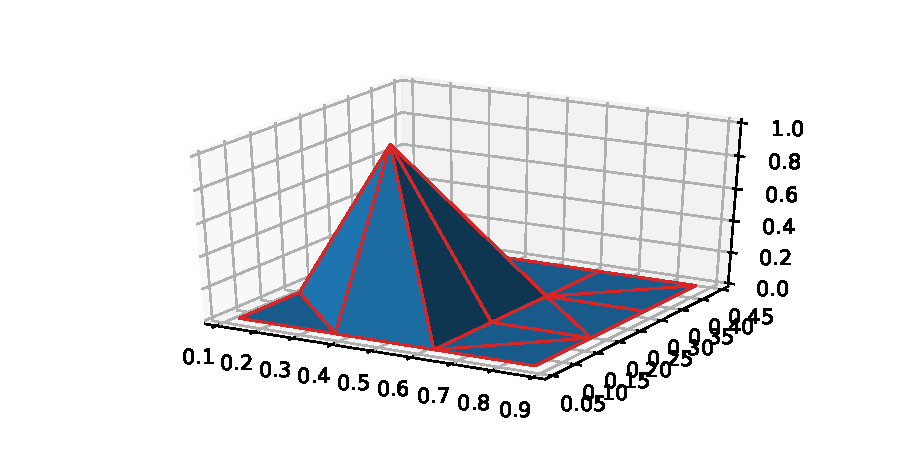
\includegraphics[width=1\textwidth]{hat1.pdf}
		\caption{A hat function .}
		\label{fig:hat1}
	\end{figure}
	Now, we demonstrate how the method works in practice. We seek a solution $u_h \in V_h$. Write this in terms of the basis functions: $u_h = \sum_{i=1}^n u_i^* \phi_i$. Now, \eqref{eq:galerkin} can be written as an equation with a solution vector with real coefficients: Find $\pmb{u}^*$ in $\mathbb{R}^n$ such that
	\begin{equation}\label{eq:fem system}
		\begin{gathered}
			\sum_{i=1}^n u_i^*  a(\phi_i,\phi_j) = b(\phi_j).
		\end{gathered}
	\end{equation}
	So we get a system of linear equations $A\pmb{u}^* = \pmb{b}$, where we have one equation for each interior node. If we solve \eqref{eq:variational poisson}, our variatonal problem, and also matrix, will be symmetric. The matrix is then often called a \emph{stiffness matrix}. These names originated from mechanics and structural analysis, where the solution represents displacement and the force function represents load. The stiffness matrix is also sparse, which is a very important property when designing algorithms to solve it.\par
	With the setup described in this section, the degrees of freedom are the same as the dimension of $V_h$. If we in definition \ref{def:linear ansatz} instead had chosen a space of quadratic polynomials on each element, we hade gained three degrees of freedom on each element. In this thesis we focus on linear finite elements because we do not gain anything from increasing regularity, as the solutions are not expected to be very regular. 
	\section*{Implementation}
	\addcontentsline{toc}{section}{Implementation}
	In this section we explain the most important parts of the algorithm for discretizing elliptic PDE's with linear triangular elements. We consider the homogenous elliptic model problem \eqref{eq:variational poisson} in two dimensions with $\pmb{K} = \pmb{I}$. The procedure goes as follows:
	\begin{enumerate}
		\item Make a triangulation of the domain. This can be done in a number of different ways, see chapter 4 of Knabner \cite{Knabner}. If we have $N$ nodes, our triangulation would be stored as a $N \times 2$ array of floats, being the coordinates of the nodes. And a $E\times 3$ array of ints beieng the elements, where each entry is the index of a coordinate in the coordinate matrix, E is the number of elements.
		\item Allocate space for the $N \times N$ stiffness matrix $\pmb{A}$ and the $N \times 1$ source vector $\pmb{b}$.
		\item Define the basis functions on a reference element, this is also called the shape functions, see figure \ref{fig:reference element} and \eqref{eq:shape functions}. Also compute the gradients of the shape functions. 
		\begin{equation}
			\begin{gathered}\label{eq:shape functions}
				N_1(x,y) = 1-x-y\\
				N_2(x,y) = x\\
				N_3(x,y) = y
			\end{gathered}
		\end{equation}
		\begin{figure}[H]
			\centering
			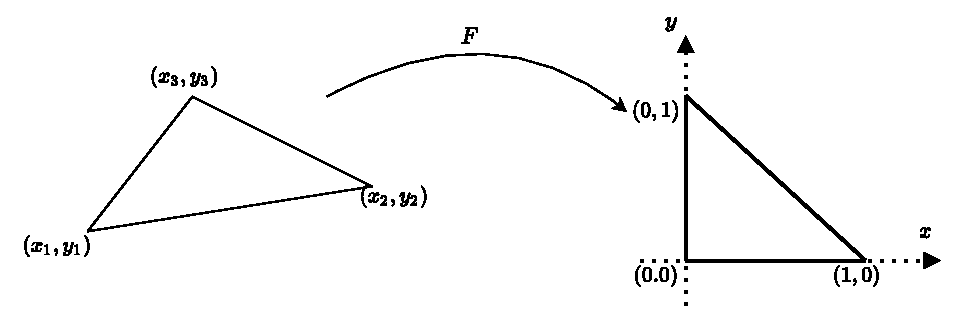
\includegraphics[width=0.85\textwidth]{reference element.pdf}
			\caption{The map $F$ from element $K$ to the reference element $\hat{K}$.}
			\label{fig:reference element}
		\end{figure}
		\item Loop trough the elements. For each element $K$ compute the affine linear map that maps it to the reference element. That means we want to find $B\in \mathbb{R}^{2\times 2}$ and $d\in \mathbb{R}^2$ such that 
		\begin{equation}
			\begin{aligned}
				F: K &\rightarrow \hat{K}\\
				x &\mapsto B x + d
			\end{aligned}
		\end{equation}
		To achieve this we set up a system of equations inspired by figure \ref{fig:reference element}
		\begin{gather}\label{eq:find_Bd}
			\begin{pmatrix}
				x_1 & y_1 & 1\\ 
				x_2 & y_2 & 1\\ 
				x_3 & y_3 & 1
			\end{pmatrix}\begin{pmatrix}
				b_{1,1} & b_{2,1}\\ 
				b_{1,2} & b_{2,2}\\ 
				d_1 & d_2
			\end{pmatrix}=
			\begin{pmatrix}
				0 &0 \\ 
				1& 0\\ 
				0 &1 
			\end{pmatrix}
		\end{gather}
		So for each element we solve \eqref{eq:find_Bd} for $B$ and $d$, that means computing an inverse of a three by three matrix and a matrix product. Note that this only needs to be done once and could be done in a preprocessing step. \par
		Now that we have $T$, we do the following on the element:
		\begin{enumerate}
					\item Use the map and the shape functions to evaluate $a(\phi_i,\phi_j)|_K$  for $1\leq i,j \leq 3$. Note that for $u: K \rightarrow \mathbb{R}$
			\begin{equation}
				\nabla^T_{\hat{x}} u(F^{-1}(\hat{x})) = \nabla^T_{x}u(F^{-1}(\hat{x}))\nabla^T_{\hat{x}} F^{-1}(\hat{x}) =\nabla^T_{x}u(F^{-1}(\hat{x})) B^{-1}
			\end{equation}
			This gives an expression for the derivative on an element expressed as a derivative in the reference element coordinate
			\begin{equation}
				\nabla_{x}u(F^{-1}(\hat{x})) = B^T \nabla_{\hat{x}} u(F^{-1}(\hat{x}))
			\end{equation}
			Now we can compute the product of the gradients of the bassis functions on an element.
			\begin{equation}\label{eq:elementgradient}
				\begin{aligned}
					a(\phi_i,\phi_j)|_K &= \int_K (\nabla \phi_i)^T \nabla \phi_j dx\\
					&= \int_{\hat{K}} (\nabla_x \phi_i(F^{-1}(\hat{x})))^T\nabla_x \phi_j(F^{-1}(\hat{x})) |\text{Det}(J(F^{-1}))|d\hat{x}\\
					&=\int_{\hat{K}}(B^T \nabla_{\hat{x}}\phi_i (F^{-1}(\hat{x})))^TB^T \nabla_{\hat{x}}\phi_j (F^{-1}(\hat{x})) |\text{Det}(B^{-1})|d\hat{x}\\
					&=\int_{\hat{K}} (\nabla_{\hat{x}}N_i(\hat{x}))^TB^TB\nabla_{\hat{x}} N_j(\hat{x}) |\text{Det}(B^{-1})|d\hat{x}\\
					&= \frac{1}{2} (\nabla_{\hat{x}}N_i(\hat{x}))^TB^TB\nabla_{\hat{x}} N_j(\hat{x}) \frac{1}{|\text{Det}(B)|}
				\end{aligned}
			\end{equation}
			So for each element we evaluate the last line of \eqref{eq:elementgradient} for all(9) combinations of $i$ and $j$ on the element 
			and add this to $\pmb{A}_{i,j}$. This approach is called \emph{element-based assembling}, and $\pmb{A}_{i,j} = \sum_{K\in \mathcal{N}(i)} a(\phi_i,\phi_j)|_K$, where $\mathcal{N}(i)$ is the set of all elements that contain node $i$.
			\item In almost the same way we compute $b(\phi_i)|_K$ and add this to $\pmb{b}_i$. As in \eqref{eq:elementgradient} we compute the integral on the reference element:
			\begin{equation}
				\begin{aligned}
					b(\phi_i)|_K &= \int_{\hat{K}} f(F^{-1}(\hat{x})) \phi_i(F^{-1}(\hat{x})) \frac{1}{\text{Det}(B)}d\hat{x}\\
					&= \int_{\hat{K}}\hat{f}(\hat{x}) N_i(F^{-1}(\hat{x}))\frac{1}{\text{Det}(B)}d\hat{x}\\
					&\approx \frac{1}{\text{Det}(B)} \sum_k \omega_k \hat{f}(\hat{p}_k) N_i(\hat{p}_k)
				\end{aligned}
			\end{equation}
			Where $\hat{f}:= f(F^{-1}(\hat{x}))$ and $\left \{ (\omega_k,\hat{p}_k) \right \}_k$ defines a \emph{quadrature rule}. We will see later that this quadrature rule can be chosen in different ways, for higher order finite elements this may even affect the convergenec behauviour. 
		\end{enumerate}

		\item Loop through the nodes $x_j$ at the boundary and set $\pmb{A}_{j,i}=\delta_{ij}$, $b_j = 0$

	\end{enumerate}
	\begin{remark}
		If we have inhomogeneous Dirichlet boundary conditions this is in practice done the same way as in the homogenous case, eliminating the degrees of freedom on the boundary. For Neumann conditions one has to evaluate integrals along the boundary as in \eqref{eq:inhomogenous poisson weak}, using one-dimensional elements.
	\end{remark}
	\section*{Convergence}
	\addcontentsline{toc}{section}{Convergence}
	
	In this section, we review the most important concepts in studying the convergence fo FEM, for a detailed discussion see \cite{Knabner}.
	The starting point of convergence estimates for the finite element method already described are \textbf{Cèa's lemma}. 
	\begin{theorem}
		Let $u$ solve the variational problem \eqref{eq:variational problem} and $u_h$ solve the corresponding Galerkin approximation \eqref{eq:galerkin}, where the bi linear form $a$ is bounded and coercive. Then we have:
		\begin{equation}
			\left \| u-u_h \right \|_V \leq \frac{C_b}{C_c}\text{min} \left \{ \left \| u-v_h \right \|: \ v_h \in V_h \right \}.
		\end{equation}
		
	\end{theorem}
	\begin{proof}
		By the coercivity and linearity of $a(\cdot,\cdot)$ we have:
		\begin{equation*}
			C_c \left \| u-u_h \right \|^2_V \leq a(u-u_h,u-u_h) = a(u-u_h,u-v_h) + a(u-u_h, v_h - u_h).
		\end{equation*}
		The last term equals zero, since both $u$ and $u_h$ solves the variational problem in $V_h$: $v_h-u_h = v \in V_h$ and $a(u-u_h,v) = a(u,v)-a(u_h,v) = b(v)-b(v) = 0$, this is called \emph{Galerkin orthogality}. Hence we only need to use the boundedness of $a(\cdot,\cdot)$:
		\begin{equation*}
			C_c \left \| u-u_h \right \|^2_V \leq a(u-u_h,u-u_h) \leq C_b \left \| u-u_h \right \|_V \left \| u-v_h \right \|_V.
		\end{equation*}
		We divide by $C_c$ and $\left \| u-u_h \right \|_V$ and take the infimum over $v_h \in V_h$:
		\begin{equation*}
			\left \| u-u_h \right \|_V \leq \frac{C_b}{C_c} \text{inf} \left \{ \left \| u-v_h \right \|_V: v_h \in V_h \right \}.
		\end{equation*}
		By (Cheney \cite{Cheney}, page 64, theorem 2), as $V_h$ is closed and convex subspace of a Hilbert space, there exist an unique element of $V_h$ closest to $u$ and minimum is attained.  
	\end{proof}
	Hence the solution to Galerkin problem is the best in the subspace $V_h$ up to a constant. We can therefore study convergence rate estimates for a suitable comparison element in $V_h$. In one dimension it is easy to picture what this comparison element might be, see figure \ref{fig:1dinterpolation}. A direct proof with techniques from calculus is possible in this case.\\
	\begin{figure}[H]
		\centering
		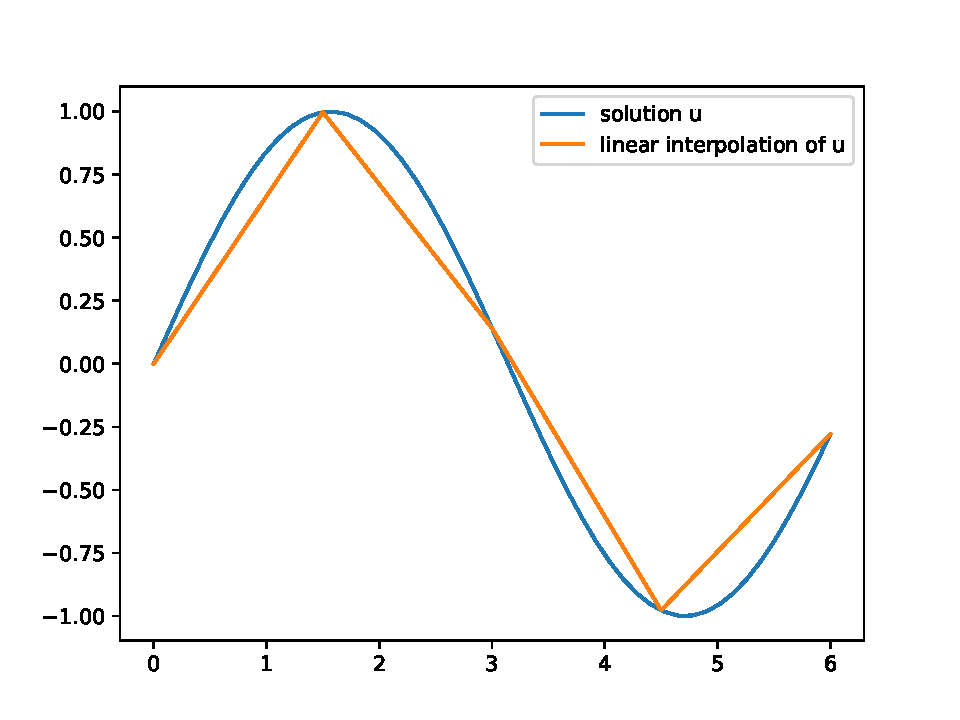
\includegraphics[width=0.7\textwidth]{interpolation.pdf}
		\caption{The unique linear interpolation of a function in one dimension.}
		\label{fig:1dinterpolation}
	\end{figure}
	The idea for more dimensions are the same, to be precise we define the interolation operator.
	\begin{definition}[Global interpolation operator]		\label{def:global_interpolator}
		\begin{gather*}
			I_h:C(\overline{\Omega}) \rightarrow V_h \\
			v \mapsto \sum_{i}v(n_i) \phi_i
		\end{gather*} 
	Where $\left\{ n_i\right \}_i$ are the nodes and $\left\{ \phi_i\right \}_i$ the corresponding basis functions.

	\end{definition}
	\begin{remark}
		The global interpolator operator \ref{def:global_interpolator} maps from continuous functions, so we need to make sure our solution is continuous. By the Sobolev embedding theorem, (Evans \cite{evans10},page 286) we are okay if our space dimension is below three and $u \in H^k(\Omega)$ for $k\geq 2$.
	\end{remark}
	Hence, in the setting of the model problem \eqref{eq:variational poisson}, we hope to reach an estimate on the form
	\begin{equation}\label{eq:energy norm estimate}
		\left \| u-u_h \right \|_{1} \leq C \left \| u-I_h(u) \right \|_{1}\leq C^* h^{k}|u|_{k+1}
	\end{equation}
	Where $h$ is the maximum diameter of the elements in the triangulation, and $k$ is the polynomial degree on the ansatz space.
	This bound is indeed attainable if we make sure the triangles in our triangulation have maximum angle less than $\pi$.
	In chapter 3.4 of Knabner \cite{Knabner}, there is a detailed proof of \eqref{eq:energy norm estimate}.\\
	Note that this means that our linear finite element method has a linear convergence in the $\left \| \cdot \right \|_1$ norm, if our variational problem admits a solution with sufficient regularity. We tie these observations together in a theorem:
	\begin{theorem}[energy norm estimate]\label{th:energy error estimate}
		Consider a finite element discretization as described by \eqref{eq:fem system} in $\mathbb{R}^d$ for $d\leq 3$ on a family of triangulations with an uniform upper bound on the maximal angle. Suppose we have a linear ansatz space as in \ref{def:linear ansatz}, then
		\begin{equation}
			\left \| u-u_h \right \|_{1}\leq C h|u|_{2}.
		\end{equation}
	\end{theorem}
	Often we are happy with a convergence rate estimate in the $\left \| \cdot \right \|_0$ norm, which do not meassure an error in the approximation of the derivative. We then expect a better convergence rate, as can be shown by the \emph{duality trick}. We consider the dual prbolem of our variational problem \eqref{eq:variational poisson}: $a(v,u_f) = \left \langle f,v\right \rangle_0$, and assume some uniqueness and stability of the solution $u_f$ of this. 
	\begin{theorem}[$L^2$ estimate]
		Suppose the situation of theorem \ref{th:energy error estimate} and assume there exist an unique solution to the adjoint problem with $| u_f| \leq C \left \|f \right \|_0$, then there exist a constant $C^*$ such that:
		\begin{equation}
			\left \| u - u_h \right \|_0 \leq C^* h \left \| u- u_h \right \|_1.
		\end{equation}
	\end{theorem}
	See \cite{Knabner} for a proof. When it comes to the assumption on the dual problem, this is satisfied for our elliptic model problem \ref{eq:poisson}. If we put the last two theorems together we obtian quadratic convergence in the $L^2$ norm
	\begin{remark}
		In this chapter we have only discussed the convergence behaviour of the solution to the Galerkin problem \eqref{eq:galerkin}. In practice, one often only solves this approximately. For example the term  $b(v_h)=\int_{\Omega}fv_h \ dx$ is impossible to evaluate exactly for most source terms $f$. We will later see error estimates with this taken into account.
	\end{remark}
	\section*{Stability}
	\addcontentsline{toc}{section}{Stability}
	A stability property for the solution of the Galerkin problem \eqref{eq:galerkin} follows from remark \eqref{rm:stability}:
	\begin{equation*}
		\left \| u_h \right \|_{H_0^1} \leq \frac{1}{C_c}\left \| b \right \|_{H_0^{1'}}
	\end{equation*}
	\todo[inline]{Write more about stability properties of FEM, so that one later can compare with stability properties of the FVM methods.}
	
	

\end{document}